\chapter{Overview of the hardware}

\section{Introduction}
The magnetometer is designed for low-power operation, simple
installation and ease of construction. The entire design is open
source, allowing anyone with reasonable soldering ability to construct
one.

The magnetometer has two parts, the interfacing unit, which is fitted
onto the Raspberry Pi's \gpio\ expansion header, and the sensor
head. Both parts should be located outdoors, away from buildings, cars
and other sources of human disturbance. 

\begin{figure}
  \centering
  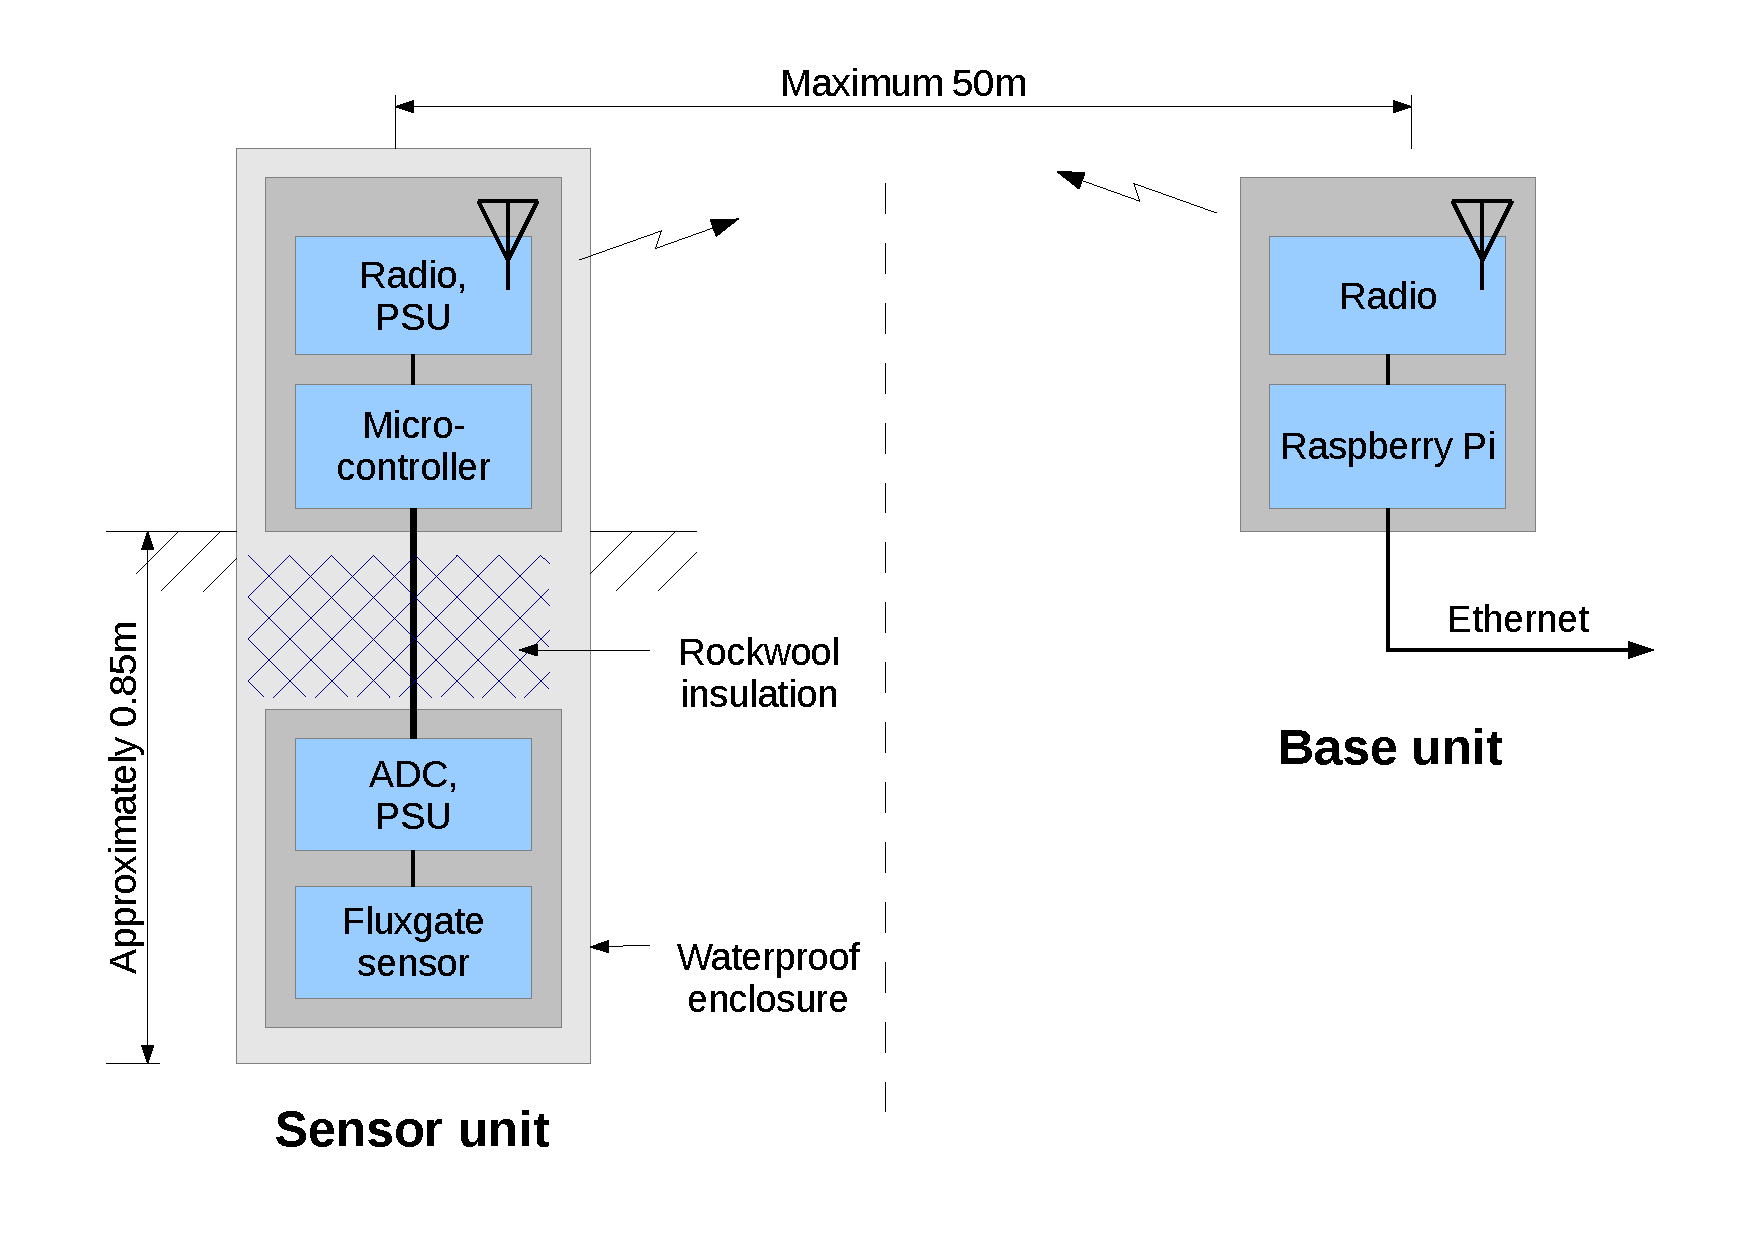
\includegraphics[keepaspectratio,width=\textwidth]{%
    raspi-mag/images/system-overview}
  \caption[System overview]%
  {System overview.}
  \label{fig:system-overview}
\end{figure}

